\section{Results}
\label{sec:results}

In the following we report and analyze results on the experiments described in the previous section. 

\subsection{Representation Modules}
% figures showing the different results of repr modules
% qualitative analysis

We begin by qualitatively analyzing the reconstructions created by the variational autoencoder (VAE), the Janus architecture and the Cerberus architecture.

\begin{figure}[t!]
	\centering
	\begin{subfigure}{0.6\columnwidth}
		\centering
		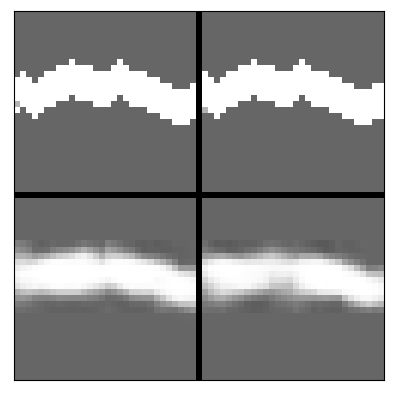
\includegraphics[width=\linewidth]{img/janus_tunnel_recon.png}
		\caption{Janus}
		\label{subfig:janus_reconstruction}
	\end{subfigure}%
	~ 
	\begin{subfigure}{0.3\columnwidth}
		\centering
		
\includegraphics[width=\linewidth]{img/cvae_tunnel_recon.png}
		\caption{CVAE}
		\label{subfig:cvae_reconstruction}
	\end{subfigure}
	
	
	\begin{subfigure}{0.9\columnwidth}
		\centering
		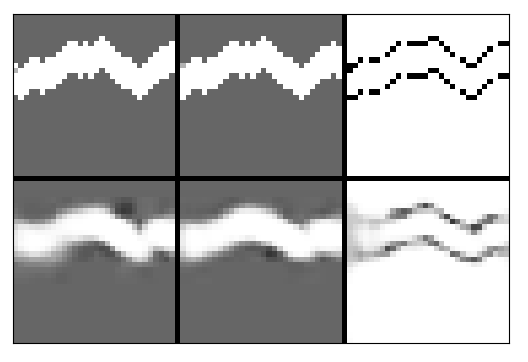
\includegraphics[width=\linewidth]{img/cerberus_tunnel_recon.png}
		\caption{Cerberus}
		\label{subfig:cerberus_reconstruction}
	\end{subfigure}

	\caption{Reconstruction of the different representation learners performing over the Tunnel task. For each architecture the ground-truth (upper images) and the reconstructions (lower images) are depicted.}
	\label{fig:repr_learner_reconstructions}
\end{figure}

In Figure \ref{fig:repr_learner_reconstructions}
    
\subsection{Policy Learner}
The results for the different tasks were taken from a point during a 50,000 episode training where intermediate performance was maximal. This avoids taking the policy in a state where the agent currently reconsiders its solution to potentially find a better one.

\begin{table}[]
\centering
\begin{tabular}{@{}lllll@{}}
\toprule
\textbf{Task} & \textbf{$\mu_r$} & \textbf{$\widetilde{r}$} & \textbf{episodes} & \textbf{baseline} \textbf{$\mu(r)$} \\ \midrule
Race & $2799.1$ & $2265$ & $36,000$ & 472\\
Tunnel &  &  & & 120\\ 
Pathing & -480 & -480 & 10,000 & -8988\\ \bottomrule
\end{tabular}
\caption{Performance of the DDQN without autoencoder loss but using a convolutional encoder. Results are given as arithmetic mean $\mu_r$ and median $\widetilde{r}$. Baseline results are using a random policy and therefore the absolut minimum performance. For the Racing and Tunnel task, maximum performance is 5000, while for Pathing -480 is the best score achievable.}
\label{my-label}
\end{table}
    
% figure showing distribution of test results
